\documentclass[11pt, letterpaper]{article}

% Includes
\usepackage{acronym}
\usepackage{amsmath, amssymb, longtable, dcolumn}
\usepackage{bm}
\usepackage{color,soul}
\usepackage{colortbl}
\usepackage{csvsimple}
\usepackage{enumitem}
\usepackage{fancyhdr}
\usepackage{fullpage}
\usepackage{hyperref}
\usepackage{IEEEtrantools} % Requires sudo apt-get install texlive-publishers texlive-publishers-doc
\usepackage{indentfirst}
\usepackage{graphicx}
%\usepackage{lgrind}
\usepackage{multirow}
\usepackage{nccmath}  % Provides \medmath to change math size
\usepackage{pdfpages}
\usepackage{siunitx}
%\usepackage{subcaption}
\usepackage[caption=false,font=footnotesize]{subfig}
%\usepackage{subfigure}
%\usepackage{stfloats}  % Written by Sigitas Tolusis
\usepackage{tabularx}
\usepackage{units}
\usepackage{url}
\usepackage{array}

% Use only one of the next two
%\usepackage{cite}
\usepackage{natbib}

% Setup
\newcommand{\doctitle}{CUSV Modeling}
\addtolength{\headheight}{2em}
\addtolength{\headsep}{1.5em}
\lhead{\doc}
\rhead{}
\setcounter{secnumdepth}{4}
\graphicspath{{images/}}
\newcommand{\capt}[1]{\caption{\small \em #1}}
\cfoot{\small Brian Bingham \today \\ \thepage}
\renewcommand{\footrulewidth}{0.4pt}

\newenvironment{xitemize}{\begin{itemize}\addtolength{\itemsep}{-0.75em}}{\end{itemize}}
\newenvironment{tasklist}{\begin{enumerate}[label=\textbf{\thesubsubsection-\arabic*},ref=\thesubsubsection-\arabic*,leftmargin=*]}{\end{enumerate}}

\makeatletter
\newcommand*{\compress}{\@minipagetrue}

% For using overleaf or local compilation
% See setting of true/false directly after \begin{document}
\newif\ifoverleaf % default is \overleaftrue

\begin{document}

% Comment out the next line if running on overleaf
\overleaffalse

% set the figure default size
\newcommand{\SF}{0.2}
\newcommand{\SFb}{0.45}
\newcommand{\SFPic}{0.45}
\newcommand{\SFPlot}{0.45}
\newcommand{\SFc}{0.25}
% Just a lazy way of setting the figure width (percentage of text width)
% 0.7 works well for 1 column
% 0.4 works well for 2 column
\newcommand{\FigWidth}{\SFb}

\newpage
% Title Page
%\setcounter{page}{1}
\begin{center}
{\huge \doctitle} \\
{\Large 1 October 2020} \\
\url{https://github.com/bsb808/OceanNotes/commits/master/cusv_model.tex}
\end{center}

\section{Overview}

\begin{figure}[hbt!]
\centering
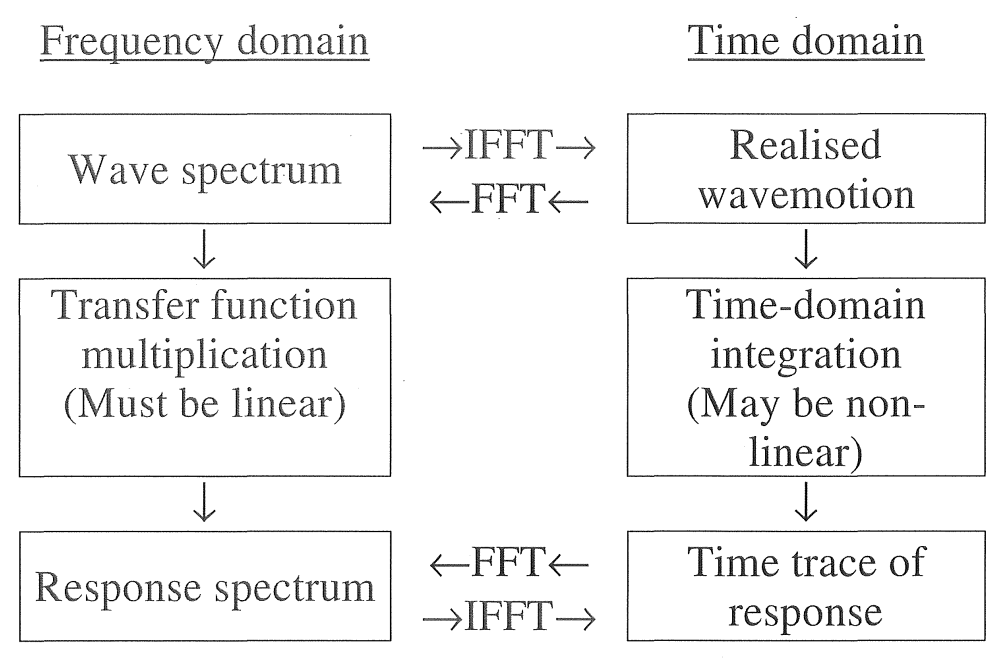
\includegraphics[width=0.6\linewidth]{images/bergdahl_roads.png}
\caption{From \cite{bergdahl09wave}}
\label{f:wave}
\end{figure}

\section{Vehicle Model}
%
To approximate the motion of a surface vehicle in the ocean environment, we adapt the six degree-of-freedom robot-like vectorial model for marine craft, proposed by \citet{fossen11handbook}, and expressed as\footnote{The rigid-body terms can be expressed equivalently using either the total vessel velocity or the velocity relative the fluid, see Property 8.1 of \citet{fossen11handbook}.  For our implementation the rigid-body terms and the hydrodynamics terms are solved for separately, and it is more direct to leverage the native physics engine in terms of total rigid-body velocity.}
\begin{equation}
\underbrace{\bm{M}_{RB}\dot{\bm{\nu}}+\bm{C}_{RB}(\bm{\nu})\bm{\nu}}_\text{rigid-body forces} + 
\underbrace{\bm{M}_A\dot{\bm{\nu}}_r + \bm{C}_A(\bm{\nu}_r)\bm{\nu}_r + 
  \bm{D}(\bm{\nu}_r)\bm{\nu}_r}_\text{hydrodynamic forces} + 
\underbrace{\bm{g}(\bm{\eta})}_\text{hydrostatic forces} 
 = \bm{\tau}_{propulsion}+\bm{\tau}_{wind}+\bm{\tau}_{waves}
\label{e:fossenmodel}
\end{equation}
where
\begin{IEEEeqnarray}{rCl}\IEEEyesnumber\label{e:estate}
    \bm{\eta} & = & [x, y, z, \phi, \theta, \psi]^T \IEEEyessubnumber \\
    \bm{\nu}  & = & [u, v, w, p, q, r]^T \IEEEyessubnumber
\end{IEEEeqnarray}
are the position and velocity vectors respectively for surge, sway, heave, roll, pitch and yaw.  The total velocity, $\bm{\nu}$, is the sum of an irrotational water current velocity, $\bm{\nu}_c$, and the vessel velocity relative to the fluid, $\bm{\nu}_r$, i.e., $\bm{\nu}=\bm{\nu}_r+\bm{\nu}_c$.  The forces and moments due to propulsion (control), wind, and waves are represented as $\bm{\tau}_{propulsion}$, $\bm{\tau}_{wind}$ and $\bm{\tau}_{waves}$.

Traditionally, surface vessel models are separated into \emph{maneuvering} models (representing the surge, sway and yaw degrees-of-freedom) and \emph{seakeeping} models (representing the heave, pitch and roll degrees-of-freedom). For the purposes of supporting the development of autonomy, it is important that the unified simulation model include \emph{both} maneuvering and seakeeping degrees-of-freedom. The maneuvering aspects of the model influence the vessel steering and control portion of the autonomy solution. The inclusion of the seakeeping aspect of the model is critical for exercising the sensory perception portion of the autonomy solution.

\section{Rigid-Body Terms}

We assume that the principal axis of inertia can be consider to be coincident with the center-of-mass of the vessel.  The vessel is symmetric about the $x-z$ plane (left-right symmetry), which implies that $I_{xy}=I{yx}=0$.  We also simplify by considering the vessel to be symmetric about the $x-y$ plane (top-bottom symmetry) such that $I_{xz}=0$.  The result is a diagonal inertia matrix.
\begin{equation}
\bm{M}_{RB}= \left[ 
\begin{array}{ccccccc}
m & 0 & 0 & 0 & 0 & 0 \\
0 & m & 0 & 0 & 0 & 0 \\
0 & 0 & m & 0 & 0 & 0 \\
0 & 0 & 0 & I_{xx} & 0 & 0 \\
0 & 0 & 0 & 0 & I_{yy} & 0 \\
0 & 0 & 0 & 0 & 0 & I_{zz} 
\end{array} \right].
\end{equation}
and a Coriolis-centripetal matrix
\begin{equation}
\bm{C}_{RB}(\bm{\nu})= \left[ 
\begin{array}{ccccccc}
  0 & 0 & 0 & 0 & mw & -mv \\
  0 & 0 & 0 & -mw & 0 & mu \\
  0 & 0 & 0 & mv & -mu & 0 \\
  0 & mw  & -mv & 0 & I_{zz}r & -I_{yy}q \\
  -mw & 0 & mu & -I_{zz}r & 0 & I_{xx}p \\
  mv & -mu & 0 & I_{yy}q & -I_{xx}p  & 0
\end{array} \right].
\end{equation}

\subsection{Parameter Estimation}

\begin{itemize}
\item Mass is calculated based on an estimate of draft, the effective length and the cross-section of a circle segment.  The value is consistent specifications of similar vessels.
\item Moments of inertia are based on an effective cylindrical model
\end{itemize}

\begin{table}
\renewcommand{\arraystretch}{1.3}
\caption{Mass properties}
\label{t:example}
\centering
\begin{tabular}{crll}
  \hline \hline
  Parameter & Value & Units & Description \\
  \hline  \hline
  \multicolumn{4}{c}{Given Values} \\
  \hline
  $L$ & 12.2 & \unit[]{m} & Length \\
  $B$ & 3.34 & \unit[]{m} & Beam \\
  $\rho$ & 1,024 & $\unit[]{kg/m^3}$ & Density of seawater \\
  \hline \hline \multicolumn{4}{c}{Estimated Values} \\
  \hline
  $T$ & 1.2 & \unit[]{m} & Draft \\
  \hline \hline \multicolumn{4}{c}{Calculated Values} \\
  \hline
  $A_{wp}$ & 35 & $\unit[]{m^2}$ & Waterplane area \\
  $\nabla$ & 32 & $\unit[]{m^3}$ & Displaced volume \\
  $m$ & 33,000 & $\unit[]{kg}$ & Mass \\
  $I_{xx}$ & 20,700 & $\unit[]{kg\cdot m^s}$ & Moment of inertia, roll \\
  $I_{yy}=I_{zz}$ & 420,000 & $\unit[]{kg\cdot m^s}$ & Moment of inertia, pitch and yaw \\
  \hline
\end{tabular}
\end{table}

\section{Hydrodynamic Terms}\label{s:hydro}
%
The hydrodynamic forces in \eqref{e:fossenmodel} include the added mass terms due to the inertia of the surrounding fluid and hydrodynamic damping terms due to the vehicle interacting with the surrounding fluid. The terms are captured using coefficients, typically referred to as hydrodynamic derivatives, and expressed using SNAME (1950) notation \citep{fossen11handbook}.

The added mass matrix for our vehicle model is expressed as
\begin{equation}\hspace{-0.15in}
\medmath{
\bm{M}_{A}= -\left[ 
\begin{array}{cccccc}
X_{\dot{u}} & 0 & 0 & 0 & 0 & 0 \\
0 & Y_{\dot{v}} & 0 & 0 & 0 & Y_{\dot{r}} \\
0 & 0  &Z_{\dot{w}} & 0 & 0 & 0 \\
0 & 0 & 0 &K_{\dot{p}} & 0 & 0 \\
0 & 0 & 0 & 0 &M_{\dot{q}} & 0 \\
0 & N_{\dot{v}} & 0 & 0 & 0 & N_{\dot{r}} 
\end{array} \right]
}
\end{equation}
where, according to \citet{fossen11handbook} we can assume $N_{\dot{v}} = Y_{\dot{r}}$ for a slow moving surface ship.


The surge, sway, yaw components of our model match the maneuvering model used by \citet{sarda16station}. For the heave, roll, pitch components, we follow the six degree-of-freedom coupled motion maneuvering model presented by \citet{fossen11handbook} that only contains the diagonal terms for these components. As noted by \citet{fossen11handbook}, the off-diagonal elements of the added mass matrix, $\bm{M}_{A}$, will be small compared to the diagonal elements for most hullforms.


Once the added mass terms that make up $\bm{M}_{A}$ are chosen, the derivation by \citet{imlay61complete} provides the Coriolis-centripetal added mass terms that result. The Coriolis-centripetal added mass matrix is expressed using the same hydrodynamic derivatives from $\bm{M}_{A}$. The resultant matrix is
\begin{equation}
    \medmath{\bm{C}_{A}(\bm{\nu}_r)=
    \left[ 
    \begin{array}{cccccc}
        0 & 0 & 0 & 0 & -Z_{\dot{w}}w_r & Y_{\dot{v}}v_r+Y_{\dot{r}}r \\
        0 & 0 & 0 & Z_{\dot{w}}w_r & 0 & -X_{\dot{u}}u_r\\       
        0 & 0 & 0 & -Y_{\dot{v}}v_r & X_{\dot{u}}u_r & 0 \\
        0 & -Z_{\dot{w}}w_r & Y_{\dot{v}}v_r & 0 & -N_{\dot{r}}r_r & M_{\dot{q}}q_r \\
        -Z_{\dot{w}}w_r & 0 & -X_{\dot{u}}u_r & N_{\dot{r}}r_r & 0 & -K_{\dot{p}}p_r \\
        -Y_{\dot{v}}v_r - Y_{\dot{r}}r & X_{\dot{u}}u_r & 0 & -M_{\dot{q}}q_r & K_{\dot{p}}p_r & 0 
    \end{array}
    \right].}
\end{equation}

Since the terms of the maneuvering portion of our unified model are chosen to match those of \citet{sarda16station}, we simply used their theoretical expressions to estimate the values for $X_{\dot{u}}$, $Y_{\dot{v}}$, $N_{\dot{r}}$, and $Y_{\dot{r}}$. To estimate the added mass terms in the seakeeping portion of our model we used the previous work of \citet{greenhow88added} involving the study of added mass and damping of partially submerged horizontal cylinders in heave and sway. From their work we were able to directly estimate the heave added mass, $Z_{\dot{w}}$, by assuming that each pontoon could be represented by a circular cylinder. For the roll and pitch added mass, we assumed that half of this added mass acted at half the beam, for roll, and a quarter of the length, for pitch.

The hydrodynamic damping includes forces due to radiation-induced potential damping, skin friction, wave drift damping, vortex shedding and lifting forces \citep{fossen11handbook,krishnamurthy05modeling}.  These effects are aggregated in the hydrodynamic damping matrix 
\begin{equation}
\bm{D}(\bm{\nu}_r) = \bm{D}_l+\bm{D}_n(\bm{\nu}_r)
\end{equation}
expressed as a sum of linear and quadratic terms:
\begin{equation}
  \medmath{
\bm{D}_l= -\left[ 
\begin{array}{cccccc}
X_{u} & 0     & 0     & 0     & 0     & 0\\
0     & Y_{v} & 0     & 0     & 0     & Y_{r}\\
0     & 0     & Z_{w} & 0     & 0     & 0 \\
0     & 0     & 0     & K_{p} & 0     & 0 \\
0     & 0     & 0     & 0     & M_{q} & 0 \\
0     & N_{v} & 0     & 0     & 0     & N_{r}
\end{array} \right]
}
\label{e:D}
\end{equation}
and
\begin{equation}\label{e:D_n}
  {
    \bm{D}_n(\bm{\nu}_r) =
    -\left[ 
      \begin{array}{cccccc}% *** did an ad-hoc horizontal spacing fix here; perhaps there's a more elegant solution
          X_{u|u|}|u_r| & \hspace{-0.25in}0 & 0 & 0 & 0 & \hspace{-0.10in}0 \\
          0 & \hspace{-0.25in}Y_{v|v|}|v_r| & 0 & 0 & 0 & \hspace{-0.10in}0  \\
          0 & \hspace{-0.25in}0 & 0 & 0 & 0 & \hspace{-0.10in}0   \\
          0 & \hspace{-0.25in}0 & 0 & 0 & 0 & \hspace{-0.10in}0  \\
          0 & \hspace{-0.25in}0 & 0 & 0 & 0 & \hspace{-0.10in}0  \\
          0 & \hspace{-0.25in}0 & 0 & 0 & 0 & \hspace{-0.10in}N_{r|r|}|r| 
      \end{array} \right].
  }
\end{equation}

This approximation of the hydrodynamic effects is implemented as a parameterized Gazebo plugin.  The user defines the characteristics of the vessel under test through a vessel-specific configuration file that includes the hydrodynamic derivatives.  During each time step of the simulation, the plugin is executed with access to the state of the vessel and environment.  The hydrodynamic force terms in \eqref{e:fossenmodel} are calculated based on this state information and the user-defined vessel characteristics.  The resulting force and moment values are then applied to the vessel through the Gazebo application programming interface (API) for inclusion in the next iteration of the physics engine.


\subsection{Drag Estimates}

The resistance $R$ do to any particular drag component is expressed as a drag coefficient $C_D$ were
\[
R = \frac{1}{2}C_D \rho S U^2
\]
where $S$ is the at-rest hull wetted surface and $\rho$ is the water density. The total ship drag, $C_T$ is expressed as
\[
C_T = C_W + (1+k) C_F
\]
where $C_w$ is the wave drag, $C_F$ is the frictional drag and $k$ is a form factor representing the viscous pressure drag some fraction of the frictional resistance coefficient.


\begin{table}
\renewcommand{\arraystretch}{1.3}
\caption{Hull-Form/Fineness Coefficients}
\label{t:hullform}
\centering
\begin{tabular}{llrl}
  \hline \hline
  Parameter & Symbol & Value & Units \\
  \hline  \hline
  \multicolumn{4}{c}{Given Values} \\
  \hline
  Length of waterline & $L$ & 12.2 & \unit[]{m} \\
  Beam on waterline & $B$ & 3.34 & \unit[]{m} \\
  \hline \hline \multicolumn{4}{c}{Estimated Values} \\
  \hline
  Draft &  $T$ & 1.2 & \unit[]{m} \\
  \hline \hline \multicolumn{4}{c}{Calculated Values} \\
  \hline
  Waterplane area & $A_{wp}$ & 35 & $\unit[]{m^2}$  \\
  Maximum section area & $A_X$ & 3.01 & $\unit[]{m^2}$  \\
  Midship section area & $A_M$ & 3.01 & $\unit[]{m^2}$  \\
  Wetted surface Area & $S$ & 51 & $\unit[]{m^2}$  \\
  Displaced volume & $\nabla$ & 32 & $\unit[]{m^3}$ \\
  \hline \hline \multicolumn{4}{c}{Hull-Form Coefficients} \\
  \hline
  Prismatic & $C_P = \frac{\nabla}{A_X L} $ & 0.875 &\\
  Volumetric & $C_V = \frac{\nabla}{L^3} $ & 0.018 &\\
  Maximum Section & $C_X = \frac{A_X}{BT} $ & 0.75 &\\
  Midship Section & $C_M = \frac{A_M}{BT} $ & 0.75 &\\
  Block & $C_B = \frac{\nabla}{LBT} $ & 0.66 &\\
  Vertical Prismatic & $C_{PV} = \frac{\nabla}{A_{WP}T} $ & 0.75 &\\
  Waterplane  & $C_{WP} = \frac{A_{WP}}{LB} $ & 0.875 &\\
  & $B/T$   & 2.8 & \\
  & $S/V^{2/3}$ & 5.1 \\
  \hline 
\end{tabular}
\end{table}

\begin{figure}[hbt!]
\centering
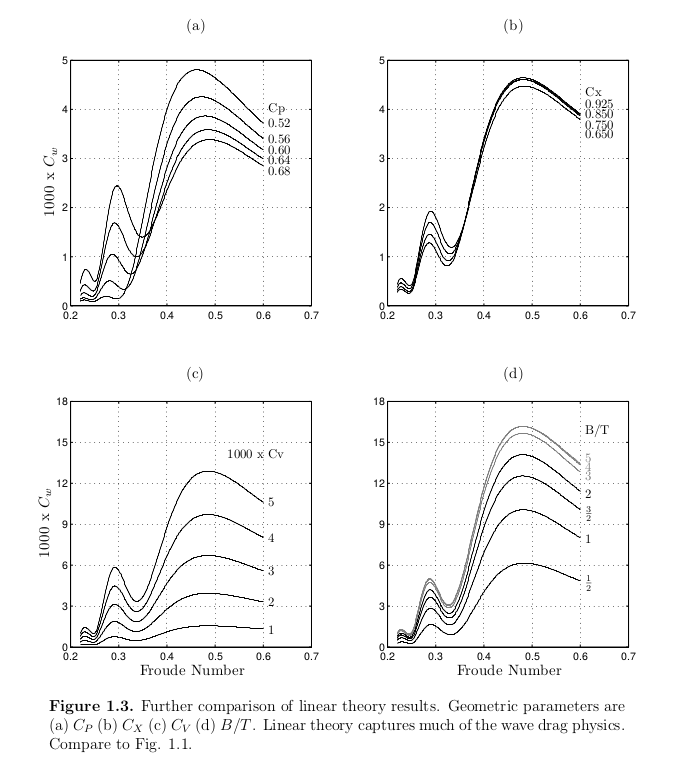
\includegraphics[width=0.6\linewidth]{drag_est.png}
\caption{\cite{read09drag}}
\label{f:drag_est}
\end{figure}


Holtrop's method suggests that the frictional drag component can be neglected for normal  \cite{holtrop82approximate,holtrop84statistical}

\begin{itemize}
\item Assume a Froude number between $Fr=0.2--0.3$, which is $U=\unit[2.2--3.3]{m/s}$.
\item Figure~\ref{f:drag_est} suggests $C_w \approx \num{1.0e-3}$.
\item Using Holtrop's method \cite{holtrop82approximate,holtrop84statistical}, we calculate $(1+k) = 1.76$
  \item Using ITTC 1957 line/method $C_F = \frac{0.075}{(log_{10}(Re)-2)^2}$ suggest that  $C_w \approx \num{2.0e-3}$ which is consistent with the guideline that the majority of the hull's total resistance is due to water friction at slow speeds.
  \end{itemize}
The result is $C_T = \num{4.5e-3}$, the total resistance force is
\[
R = \frac{1}{2}C_T \rho S U^2  = (118.0) \, U^2
\]
So
\begin{itemize}
\item $X_u = 0$
\item $X_{u|u|}=\unit[118.0]{N/(m/s)^2}$
\item If similarity to VRX model holds, then
  \begin{itemize}
  \item  $Y_{u|u|}= 11.4 \cdot X_{u|u|} = \unit[1345.0]{N/(m/s)^2}$
  \item  $Z_{v|v|}= 31.2 \cdot X_{u|u|} = \unit[3680.0]{N/(m/s)^2}$
  \end{itemize}  
\end{itemize}

\section{Summary}

\begin{table}
\renewcommand{\arraystretch}{1.3}
\caption{Model Parameters}
\label{t:params}
\centering
\begin{tabular}{>{\raggedright}p{0.18\linewidth}
  >{\raggedright}p{0.2\linewidth}
  rl
  >{\raggedright}p{0.25\linewidth}}%{p{1.5in}p{1.5in}rlp{1.5in}}
  \hline \hline
  Parameter & Description & Value & Units & Method \tabularnewline
  \hline
  $m$ & Mass & 33,000 & $\unit[]{kg}$ & Displacement estimate based on geometry \tabularnewline
  $I_{xx}$ & MOI-roll & 20,700 & $\unit[]{kg\cdot m^s}$ & Effective cylinder\tabularnewline
  $I_{yy}=I_{zz}$ & MOI-pitch/yaw & 420,000 & $\unit[]{kg\cdot m^s}$ & Effective cylinder \tabularnewline
  $X_{\dot{u}}$ & Added mass, surge & 0 & $\unit[]{kg}$ & Neglected \tabularnewline
  $Y_{\dot{v}}$ & Added mass, sway  & 26,000 & $\unit[]{kg}$ & Cylinder \cite{greenhow88added} \tabularnewline
  $Z_{\dot{w}}$ & Added mass, heave  & 31,000 & $\unit[]{kg}$ & Cylinder \cite{greenhow88added} \tabularnewline
  $K_{\dot{p}}=M_{\dot{q}}=N_{\dot{r}}=Y_{\dot{r}}=N_{\dot{v}}=$ & Added mass, roll/pitch/yaw   & 0 & $\unit[]{kg \cdot m^2}$ & Neglected \tabularnewline
  $X_{u}=0$ & Drag, linear, surge & 0 & $\unit[]{N/(m/s)}$ &  \cite{holtrop82approximate,holtrop84statistical,read09drag} \tabularnewline
  $X_{u|u|}$ & Drag, quadratic, surge & 118 & $\unit[]{N/(m/s)^2}$ &   \cite{holtrop82approximate,holtrop84statistical,read09drag} \tabularnewline
  $Y_{v}=0$ & Drag, linear, sway & 0 & $\unit[]{N/(m/s)}$ & Proportional to VRX model \tabularnewline
  $Y_{v|v|}$ & Drag, quadratic, sway & 1345 & $\unit[]{N/(m/s)^2}$ &  Proportional to VRX model \tabularnewline
$K_{p}, \, K_{p|p}, \, M_{q}$, $M_{q|q|}, \, N_{r}, \, N_{r|r|}$ & Drag & Various & & SIT  \tabularnewline
  \hline
\end{tabular}
\end{table}

\clearpage

\section{Frequency Domain Model}

Deduced from time-domain model via step response tests.  Identification of second-order transfer function parameters via logarithmic decrement.  The form of the second order transfer function is
\begin{equation}
  G(s) = \frac{\omega_n^2}{s^2 + 2 \zeta \omega_n s + \omega_n^2}
\end{equation}


\begin{table}[hb!]
\renewcommand{\arraystretch}{1.2}
\caption{Frequency domain system parameters}
\label{t:freq}
\centering
\begin{tabular}{llrl}
  \hline \hline
  Parameter & Symbol & Value & Units \\
  \hline  \hline
  \multicolumn{4}{c}{Heave: Figure~\ref{f:h}} \\
  \hline
  Period & $T$ & 2.0 & $\unit[]{s}$ \\
  Damping ratio & $\zeta$ & 0.13 & n/a \\
  Undamped natural freq.  & $\omega_n$ & 3.19 & $\unit[]{rad/s}$ \\
  Damped natural freq.  & $\omega_d$ & 3.16 & $\unit[]{rad/s}$ \\
  \hline \hline \multicolumn{4}{c}{Pitch: Figure~\ref{f:p}} \\
  \hline
  Period & $T$ & 1.6 & $\unit[]{s}$ \\
  Damping ratio & $\zeta$ & 0.14 & n/a \\
  Undamped natural freq.  & $\omega_n$ & 4.08 & $\unit[]{rad/s}$ \\
  Damped natural freq.  & $\omega_d$ & 4.04 & $\unit[]{rad/s}$ \\
  \hline \hline \multicolumn{4}{c}{Roll: Figure~\ref{f:r}} \\
  \hline
  Period & $T$ & 0.63 & $\unit[]{s}$ \\
  Damping ratio & $\zeta$ & 0.021 & n/a \\
  Undamped natural freq.  & $\omega_n$ & 9.92 & $\unit[]{rad/s}$ \\
  Damped natural freq.  & $\omega_d$ & 9.92 & $\unit[]{rad/s}$ \\
\end{tabular}
\end{table}

\begin{figure}[hb!]
\centering
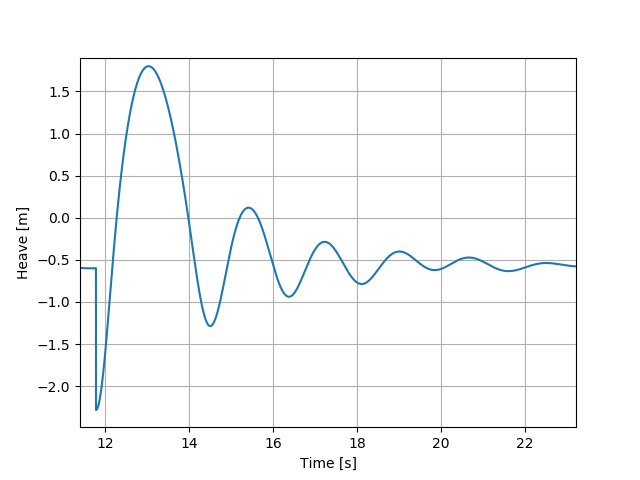
\includegraphics[width=0.6\linewidth]{./src/usv_param_est/heave_step.png}
\caption{Heave step response}
\label{f:h}
\end{figure}

\begin{figure}[hb!]
\centering
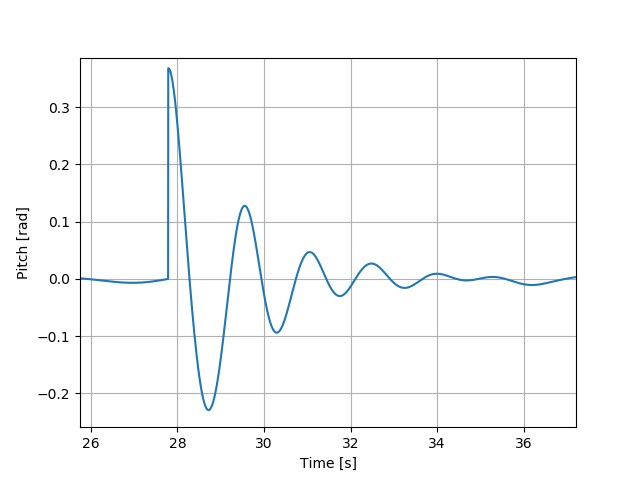
\includegraphics[width=0.6\linewidth]{./src/usv_param_est/pitch_step.png}
\caption{Pitch step response}
\label{f:p}
\end{figure}

\begin{figure}[hb!]
\centering
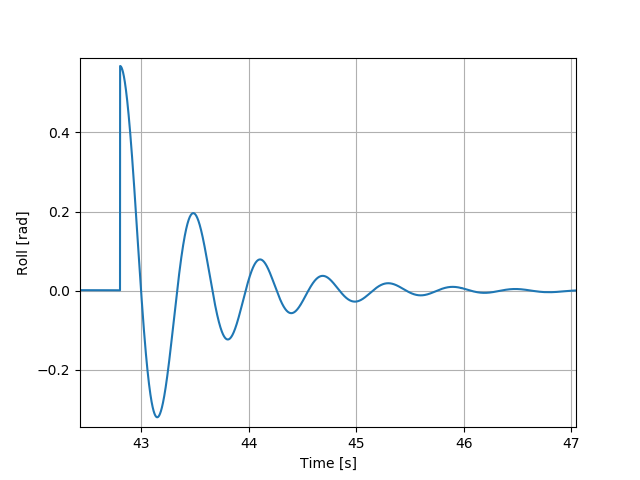
\includegraphics[width=0.6\linewidth]{./src/usv_param_est/roll_step.png}
\caption{Roll step response}
\label{f:r}
\end{figure}


\clearpage

\subsection{Spectral Metrics}

Based on wave height metrics\footnote{\url{http://www.coastalwiki.org/wiki/Statistical_description_of_wave_parameters}}.

\begin{equation}
  E[\eta^2(t)] = \sigma_{\eta}^2 = m_0 = R_{\eta \eta}(\tau=0)  =  \int_{0}^{\infty}\Gamma_{\eta \eta}(\omega) d\omega
\end{equation}
where $\eta(x,y,t)$ is the ocean height at a certain location $x,y$ as a function of time $t$, $E[]$ is the expectation operator, $\sigma_{\eta}^2$ is the variance in wave height, equivalently the zeroth moment ($m_0$) and $\Gamma_{\eta \eta}(\omega)$ is the one-sided wave height spectrum as a function of angular frequency.


\subsubsection{Wave Slope Spectra}

For deep water waves the dispersion relation $\omega = \omega(k)$ is
\begin{equation}
  \omega = \sqrt{g\,k}.
\end{equation}
Because at any time $t$ we can consider a 2D wave and the slope of that wave as
\begin{IEEEeqnarray}{rCl}\IEEEyesnumber\label{e:slope}
    \eta(x) & = & a\cos(kx) \IEEEyessubnumber \\
    \alpha(x)  = \frac{d \eta(x)}{dx}  & = & a \, k \cos(kx). \IEEEyessubnumber
\end{IEEEeqnarray}
The wave slope spectrum can be expressed as
\begin{equation}
  \Gamma_{\alpha \alpha} = k^2 \;  \Gamma_{\eta \eta}(\omega) =  \frac{\omega^4}{g^2}   \; \Gamma_{\eta \eta}(\omega)
\end{equation}

\subsubsection{Characteristic Wave Heights}

As summarized in \cite{young99wind} the propbability density function of wave heights is typically considered to follow the Rayleigh distribution
\begin{equation}
  p(H; 2\sigma_{\eta}) = \frac{H}{(2\sigma_\eta)^2} e^{-H^2/(2(2\sigma_\eta)^2)}
\end{equation}
Here $H$ is the wave height and the Rayleigh distribution scale parameter is $\sigma = 2 \sigma_\eta$.



\begin{table}[hb!]
\renewcommand{\arraystretch}{1.7}
\caption{Characteristic wave height metrics or represenatative measures of wave height}
\label{t:wavemetrics}
\centering
\begin{tabular}{lcp{0.3\linewidth}}
  \hline \hline
  Characteristic & Parameter Value & Description \\
  \hline 
  Mean & $\bar{H} = H_{1/1} =  \sqrt{2 \pi} \, \sigma_\eta = 2.51 \, \sigma_\eta$ & Average height of all waves.\\
  Root-mean-square & $H_{rms} = 2 \sqrt{2} \, \sigma_\eta = 2.83 \, \sigma_\eta$ & \\
  Significant & $H_{1/3}=H_s = 4 \, \sigma_\eta$ & Average height of the 1/3rd highest waves. \\
   & $H_{1/10} = 5.09 \, \sigma_\eta$ & Average height of the 1/10th highest waves. \\
  & $H_{1/100} = 6.67 \, \sigma_\eta$ & Average height of the 1/100th highest waves. \\
  
\end{tabular}
\end{table}

\subsection{Results}
% Set figure width
\newcommand{\RFW}{0.7}

The source for generating the analysis and figures is in the \verb+leanis_analysis+ repository at \url{https://bitbucket.org/greensightag/leanis_analysis/src/master/vessel_seakeeping/wave_spectrum_ex.py}.

\subsubsection{Wave Spectra: Wave Height and Slope}

\begin{figure}[hbt!]
\centering
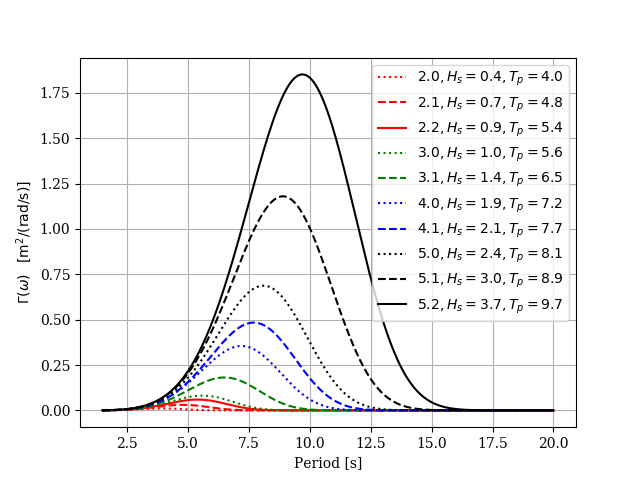
\includegraphics[width=\RFW\linewidth]{cusv/SvsT.png}
\caption{Wave height spectra vs. wave period.}
\label{f:SvsT}
\end{figure}

\begin{figure}[hbt!]
\centering
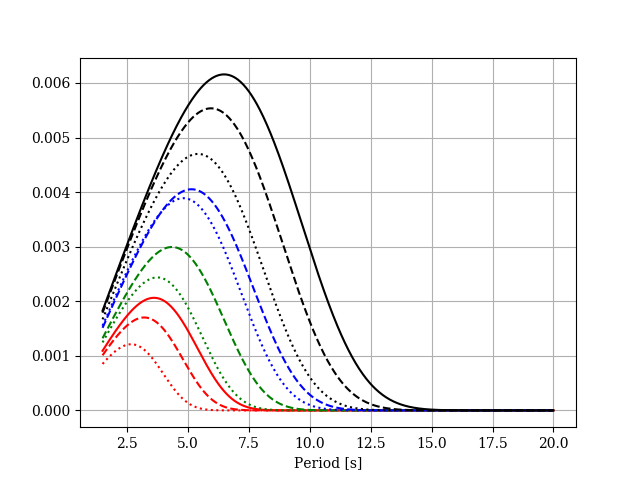
\includegraphics[width=\RFW\linewidth]{cusv/slopeVt.png}
\caption{Wave slope spectra vs. wave period.}
\label{f:slopeVt}
\end{figure}

\subsubsection{Vessel Motion Spectra: Heave, Pitch and Roll}

\begin{figure}[hbt!]
\centering
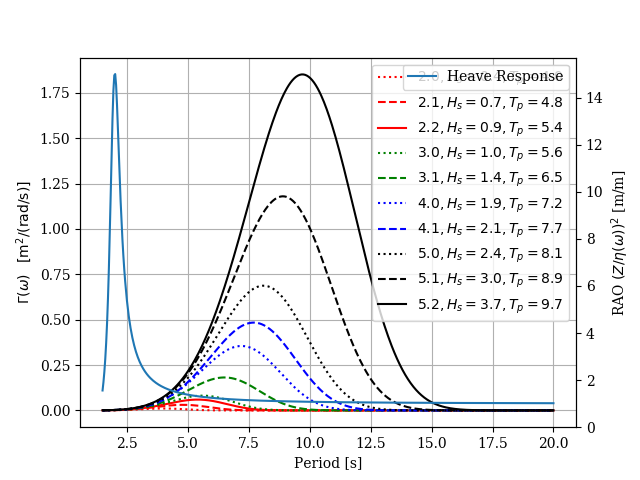
\includegraphics[width=\RFW\linewidth]{cusv/SvsTwG.png}
\caption{Wave height spectra alongside the heave response as a transfer function.}
\label{f:SvsTwG}
\end{figure}

\begin{figure}[hbt!]
\centering
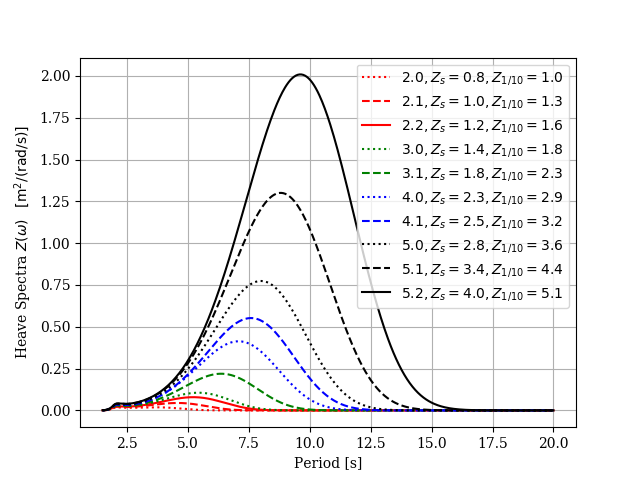
\includegraphics[width=\RFW\linewidth]{cusv/heaveresp.png}
\caption{Heave spectra and heave height metrics.}
\label{f:heaveresp}
\end{figure}

\begin{figure}[hbt!]
\centering
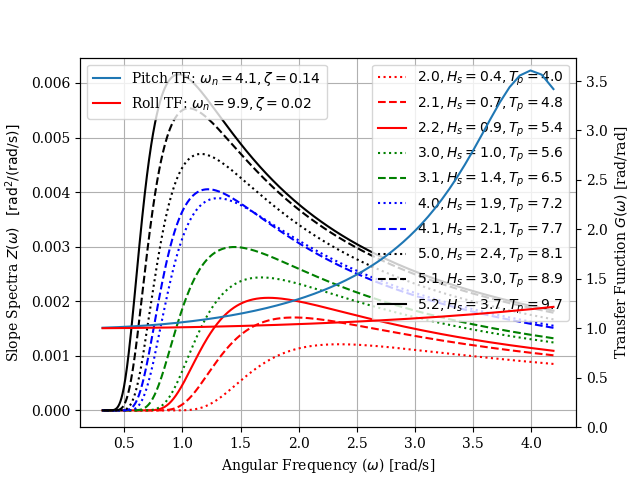
\includegraphics[width=\RFW\linewidth]{cusv/slope_respover.png}
\caption{Slope spectra alongside pitch and roll responses as transfer functions.}
\label{f:slope_respover}
\end{figure}

\begin{figure}[hbt!]
\centering
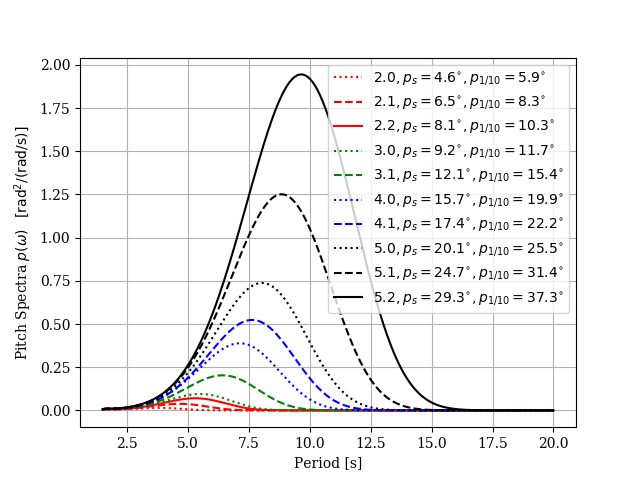
\includegraphics[width=\RFW\linewidth]{cusv/pitchresp.png}
\caption{Pitch spectra and metrics, peak-to-peak in degrees}
\label{f:pitchresp}
\end{figure}

\begin{figure}[hbt!]
\centering
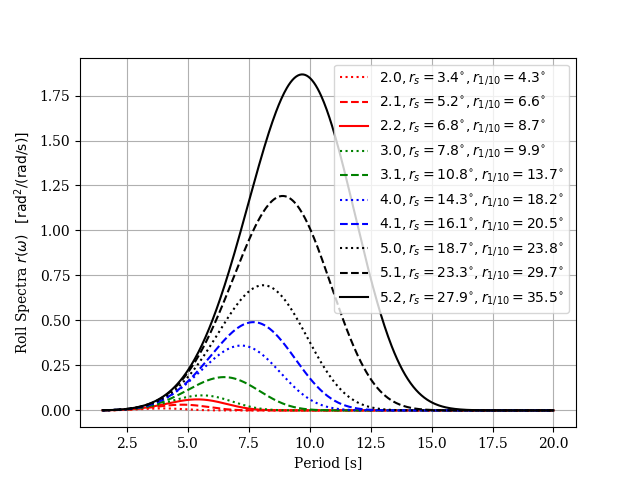
\includegraphics[width=\RFW\linewidth]{cusv/rollresp.png}
\caption{Roll spectra and metrics, peak-to-peak in degrees}
\label{f:rollresp}
\end{figure}

\clearpage

\bibliographystyle{apalike}

%\bibliography{bbing_master}

\ifoverleaf
\bibliography{bbing_master, ocean_notes}
\else
\bibliography{../latexlib/bib/bbing_master}
\fi

\end{document}

